%!TEX root = labreport.tex
%%%%%%%%%%%%%%%%%%%%%%%%%%%%%%%%%%%%%%%%%%%%%%%%%%%%%%%%%%%%%%%%%%%%%%%%%%%

\documentclass[sigconf]{acmart}

\usepackage{booktabs} % For formal tables
\usepackage{amsmath}

% Copyright
\setcopyright{none}
%\setcopyright{acmcopyright}
%\setcopyright{acmlicensed}
%\setcopyright{rightsretained}
%\setcopyright{usgov}
%\setcopyright{usgovmixed}
%\setcopyright{cagov}
%\setcopyright{cagovmixed}


% DOI
% \acmDOI{10.475/123_4}

% ISBN
% \acmISBN{123-4567-24-567/08/06}

%Conference
\acmConference[SEEMOO PhySec (Lab RDS) 2017/18]{Physical Layer Security
in Wireless Systems (Lab RDS) 2017/18}{February 2018}{Darmstadt, Germany}

\acmYear{2018}
\copyrightyear{2018}

% \acmArticle{4}
% \acmPrice{15.00}

\settopmatter{printacmref=false}

\begin{document}
\title{Reactive Jamming}

% Comment out the following for you final document
\subtitle{Lab Report}



\author{Daniel May}
\author{Simon Schmitt}
\affiliation{%
  \institution{Technische Universtit\"at Darmstadt}
}
\email{daniel\_nicolas.may@stud.tu-darmstadt.de}
\email{simon\_johannes.schmitt@stud.tu-darmstadt.de}

% The default list of authors is too long for headers.
\renewcommand{\shortauthors}{Daniel May \& Simon Schmitt}


\begin{abstract}
%  Answer the following questions with roughly one sentence each:
%
%  One-page summary:
%  \begin{itemize}
%  \item What is the topic of your main seminar paper?
%  \item What problem does it solve?
%  \item Why is that topic/problem important?
%  \item What methodologies do the authors apply?
%  \item What are the main contributions of the paper?
%  \item What are the key findings/results of the paper?
%  \end{itemize}
%  
%  Final seminar paper:
%  \begin{itemize}
%  \item What is your research question?
%  \item Why are that question and your topic important?
%  \item How did you proceed to answer the question?
%  \item What (do you think) is the answer to your question?
%  \item Give an overall opinion on your topic.
%  \item If you have results, describe them.
%  \item What is the impact of the answers to your questions?
%  \end{itemize}
This lab report presents the creation of an reactive jammer. We will describe how the frame handling
works on the WARP and how it can be used to suppress individual targeted devices or communications
respectively. At the end of this report we evaluate the performance of our jammer and discuss
possible improvements.


\end{abstract}

\maketitle

\section{Introduction}
Wireless signals, as they are used in most of today's analog or digital communications, are very
sensitive and affectable by the environment. Signals with the same frequency can interfere and
suppress each other. This effect is typically used by jammers to prevent a certain receiver from
decoding a signal. While jamming is typically associated with malicious behaviour or within military
conflicts to hinder an opposing party from exchanging information, there also exists other jamming
schemes, so called friendly jamming. Friendly jamming can be used to protect vulnerable systems from
adversarial actions, e.g., pacemakers that can be wirelessly reprogrammed. More recent work also
demonstrated that secrete key-exchanges can be realized at the physical layer utilizing a jammer.

The objective of this lab was to create a reactive WiFi jammer using the Wireless Open-Access
Research Platform (WARP). WARP is a programmable Software-Defined Radio (SDR) which provides a basic
implementation of the 802.11g WiFi standard. The architecture of the WARP allows to transmit frames
while still receiving a signal. Thus WiFi transmissions with a certain Medium Access Control (MAC)
address can be analyzed and jammed if they are matching a target address.

In comparison with existing jammers this approach is more precise as it only suppresses the signals
of a certain target, while still allowing the communication of other devices. This also results in
much lower power-consumptions, due to the smaller amount of frames that have to be jammed.

%Write a short paragraph (5-15 lines) on each of the following tasks:
%\begin{itemize}
%\item Motivate your topic in general.
%\item Why is your research question important in that field?
%\item Give one practical example.
%\item To what existing work is your topic related, what has been done there?
%\item What are the (planned) main contributions of your paper? e.g., a
%new attacker model, a summary, a comparison, \dots
%\item Give an outline of the paper: describe each of your (planned)
%sections in one sentence.
%\end{itemize}


\section{Background on the WARP}
In this Section we describe how the frame handling works on the Wireless Open-Access
Research Platform (WARP) and why there are multiple receive and transmit buffers.

The WARP is a transceiver, which means it can be used to send and receive frames respectively. This
is realized with two independent paths of circuits that are connected to a single antenna (1). 
The antenna is followed by a switch (2) to either connect to the transmit or receiver
path. At the receiving path the incoming frames are directly forwarded to the transceiver module
(4), while the signals leaving this module are amplified to a fixed gain (3). The transceiver module
controls the conversion between the complex baseband signal and the Radio Frequency (RF) using a
quadrature modulator. The next layer (5) contains the Digital-to-Analog and Analog-to-Digital
Converter, which are connected to the chips that implement the 802.11 physical layer (6). Incoming
frames are written into a RX Packet Buffer, while outgoing frames are read from the TX Packet
Buffer. Both buffers represent shared memory that is also accessible by the MicroBlaze processor (7),
which handles the MAC layer of the network interface. Whats special about the WARP, is the fact that
the processor allows to start processing while incoming frames are still being received. This
allows us to implement a reactive jammer. It is only necessary to prepare the frames used for the
jamming signal. Those frames are stored in the TX Packet Buffer and can be send as soon as a
condition matches to the incoming frame.

The JTAG port (9) is used to flash the firmware of the processor and to upload the implementation of
the reactive jammer. Any debugging messages that are written to the standard output can be observed
in a terminal that is connected to the UART to USB port (10).

\begin{figure}[tb!]
	\hfill
	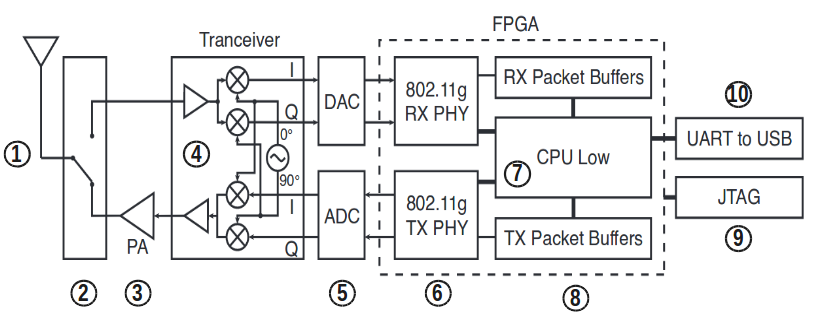
\includegraphics[width=1\linewidth]{block_diagram_warp.png}
	\caption{Block diagram of the 802.11 WARP}
	\label{fig:block_diagram_warp}
\end{figure}

\section{Implementation}

In this Section we describe how a reactive jammer can be implemented using the previous described
Wireless Open-Access Research Platform (WARP). As a development environment we used the Eclipse-based
Xilinx Software Development Kit and Putty as a terminal for the standard output. The logic is
implemented in C and executed by the CPU low of the WARP.

\pagebreak

As a first step we setup the WiFi 802.11 standard and the callback-function that are executed if a
new frame is received or needs to transmitted. 

\begin{verbatim}
	wlan_mac_low_init(WARPNET_TYPE_80211_LOW);

	// ...

	wlan_mac_low_set_frame_rx_callback((void*)frame_receive);
	wlan_mac_low_set_frame_tx_callback((void*)frame_transmit);
\end{verbatim}

In order to check for incoming frames, the wlan\_mac\_low\_poll\_frame\_rx function needs to be executed
in a loop. 

\begin{verbatim}
	while(1) {
		wlan_mac_low_poll_frame_rx();
	}
\end{verbatim}

If the RX PHY received a new frame this function will call the frame\_received function to handle the
reception. Since, we are about to implement a reactive jammer, it is of importance that the jamming
signal is send as soon as the currently received frame can be assigned to a certain transmitter.
Therefore, we added the check for the jamming condition (MAC address of the target system) to the
frame\_received function. If the condition is "true" we create the jamming signal and transmit it
using the frame\_transmit function. Notice that the transmission is started, while still
receiving the targeted signal. As a result the signal gets destroyed for other receivers.


\begin{verbatim}
	u32 frame_receive(u8 rx_pkt_buf, u8 rate, u16 length){
		mac_header_80211 header;

		while(wlan_mac_get_last_byte_index() <= 19) {
			xil_printf("");
		}

		memcpy(&header, ((void *)(RX_PKT_BUF_TO_ADDR(rx_pkt_buf)) + 
				PHY_RX_PKT_BUF_PHY_HDR_SIZE + sizeof(rx_frame_info)), 
				sizeof(header));

		if (wlan_addr_eq(header.address_1, jam_me_mac)) {
			is_pushed = 1;
			u8 pkt_buf = 0;
			mac_header_80211 header;
			header.frame_control_1 = MAC_FRAME_CTRL1_SUBTYPE_DATA;
			header.frame_control_2 = MAC_FRAME_CTRL2_FLAG_FROM_DS;
			header.duration_id = 0;
			memcpy(header.address_1, mac, 6);
			memcpy(header.address_2, mac, 6);
			memcpy(header.address_3, mac, 6);
			header.sequence_control = 0;

			memcpy((TX_PKT_BUF_TO_ADDR(pkt_buf) + 
				PHY_TX_PKT_BUF_PHY_HDR_SIZE + 
				sizeof(tx_frame_info)), 
				&header, 
				sizeof(header));
			set_tx_power(pkt_buf, TX_POWER_MAX_DBM);
			set_tx_ant_mode(pkt_buf, TX_ANTMODE_SISO_ANTA);
			frame_transmit(pkt_buf,WLAN_PHY_RATE_BPSK12, sizeof(header),NULL);
		}

		//Blocks until reception is complete
		u32 state = wlan_mac_dcf_hw_rx_finish(); 
		
		// ...
	}
\end{verbatim}


\section{Conclusion and Take-Away}

\section{Future Work}


\bibliographystyle{ACM-Reference-Format}
\bibliography{library} 

\end{document}
